\section{Theory}


The modern theory of radiation was a major development in physics at the
beginning of the $20^{\rm th}$ century. A
``black body'' is a perfect
absorber, one which completely absorbs incident electromagnetic
radiation of all frequencies and which therefore appears black. When
black bodies are heated, they emit all frequencies of radiant energy in
a characteristic spectrum.  The spectrum predicted by classical theory
did not agree with experiment -- in fact it predicted an infinite total
emitted power.  The problems in explaining the actual emission
spectrum of black bodies led Max Planck to suggest that radiant energy
is quantized, {\em i.e.}\ available only in certain discrete amounts called
``quanta'', an hypothesis that laid
the foundations for modern quantum theory.  Refer to the Thornton and Rex
reference for details of Planck's treatment.  In this experiment we will measure several characteristics of black
body radiation:

\begin{enumerate}
\item The Stefan-Boltzmann $T^4$ Law, which states
that $R$, the total power/unit area of the electromagnetic radiation
emitted by a black body, is proportional to $T^4$, where
$T$ is the absolute (Kelvin) temperature of the black body. Specifically,

\begin{equation}
\label{eq:stephan-boltzman}
R = \sigma T^4, 
 \end{equation}

where $\sigma = 5.67 \times 10^{-8 } {\rm W} {\rm m}^{-2} {\rm K}^{-4}$

This behavior cannot be explained by classical theory, and is one of the
key predictions of Planck's theory based on the
hypothesis of light quanta (i.e., photons).


\item The Inverse Square Law of Heat Radiation -- the measured intensity
of radiation emitted by a point source falls off with the square of the distance from the
source.


%\item The cosine law, which states that the measurement of the intensity of
%radiation from an aperture is proportional to $cos \alpha$ when measured at an angle $\alpha$.


\item The dependence of the intensity of radiation emitted from
different surfaces at the same temperature on characteristic features of the surfaces -- {\em e.g.}\ color, shininess.
\end{enumerate}

\section{Preliminary Questions}

%In this experiment, black body radiation is emitted from an opening in
%oven at high temperature.  Assume that the oven temperature is 500 degrees C and
%that the opening is circular with diameter 2.0 cm.
%\begin{enumerate}
%\item Use the Stefan-Boltzmann equation to calculate the power/area of the
%black body radiation emitted from the opening in the oven.
%\item Determine the area of the opening, and find the total power radiated from the opening.
%\item Use the Wien displacement law,
%\begin{equation}
%\lambda_m T = 2.898 x 10^{-3}  {\rm m} {\rm K}
%\end{equation}
%to calculate the wavelength $\lambda_m$ for which the
%electromagnetic radiation emitted by the oven has maximum power.  In
%what part of the electromagnetic spectrum is this wavelength?
%\end{enumerate}

In this experiment, black body radiation is emitted from a tungsten filament with an adjustable power supply.    The filament temperature can range from room temperature to approximately 2500 K.

\begin{enumerate}
\item Use the Stefan-Boltzmann equation to calculate the power/area of the
black body radiation emitted from the bulb for the achievable range of filament temperature.

%\item Determine the area of the opening, and find the total power radiated from the opening.

\item Use the Wien displacement law,
\begin{equation}
\lambda_m T = 2.898 x 10^{-3}  {\rm m} {\rm K}
\end{equation}
to calculate the wavelength $\lambda_m$ for which the
electromagnetic radiation emitted by the bulb has maximum power at the different values of temperature.  In
what part of the electromagnetic spectrum are these wavelengths?
\end{enumerate}


\section{Equipment}

\begin{itemize}

%\item Oven with removable blackened brass-tube cavity and table mount.
% \item Power supply (0 -- 110 V) for the oven. This is a variac connected to
%an 110 V AC outlet.
%\item Thermocouple Digital Thermometer ($-112^\circ$F --
%$1999^\circ$F, $-80^\circ$C -- $1100^\circ$C,  $\pm$1\%) with Probe (to $500^\circ$C $\pm$ %0.3\% $\pm 0.5^\circ$C)

%\item Funnel-shaped aperture with asbestos coating on back and ports for
%cooling water

\item Stefan-Boltzmann adjustable light bulb (Daedalon EH-15)

\item DC Power supply for the light bulb

\item Two multimeters to read lamp voltage and current (may be able to read directly from the power supply)

\item Moll's thermopile, a sensitive detector of
electromagnetic radiation

\item Precision digital multimeter

%\item Optical bench with movable arms and riders

\item Leslie's cube (cube with white, black, and bright and
dull metallic faces)

\item Hotplate, beaker, funnel and oven mitts
\end{itemize}

\subsection{Notes on equipment}


\begin{enumerate}
\item The glass cap covering Moll's thermopile tube must
be removed before taking heat radiation measurements. The glass cap is
a protective ``dust'' cover and will
absorb the IR radiation if left on the thermopile tube. The thermopile
responds to changes in thermal radiation within 2 or 3 seconds of the
change.


\item The voltage output from the thermopile can be translated into radiant
thermal power units by the following conversion factor: 0.16 mV output
from the thermopile is equivalent to 1 mW of measured radiant thermal
power.

\item The temperature of the filament, $T_i$ is determined by calculating the resistance, $R_i$,
\begin{equation}
R_i = R_{293} \left[ 1 + \alpha \left(T_i + 293 {\rm K} )\right)\right],
\label{eq-filamenttemp}
\end{equation}
where the temperature coefficient $\alpha = 0.0045$~K$^{-1}$ for tungsten.  The measurement of the room temperature resistance, $R_{293}$, is described below. (\em The actual room temperature may not be 293 K).   

%\item The green-yellow lead, one of three leads making up the
%oven's power cable, is the ground wire and must not be
%connected to a high potential.
\end{enumerate}

\section{Procedure }

\begin{enumerate}


\item Following Figure~\ref{fig:apparatus}, carefully align the thermopile with the bulb, 
\begin{figure}
\begin{centering}

%\subfigure{
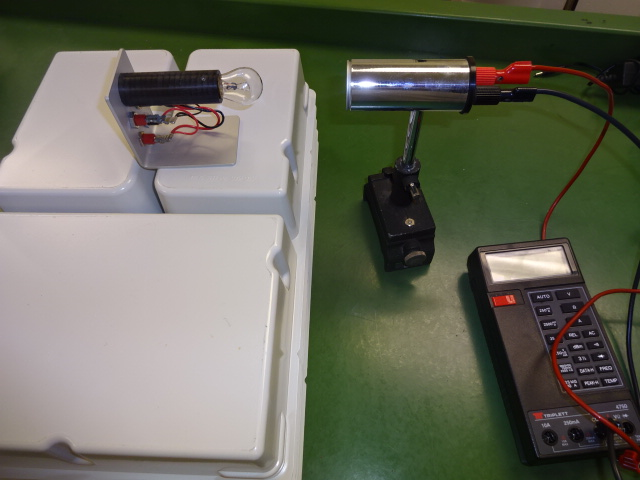
\includegraphics[width=2in]{../images/BulbThermopile.jpg}
%}
%\subfigure{
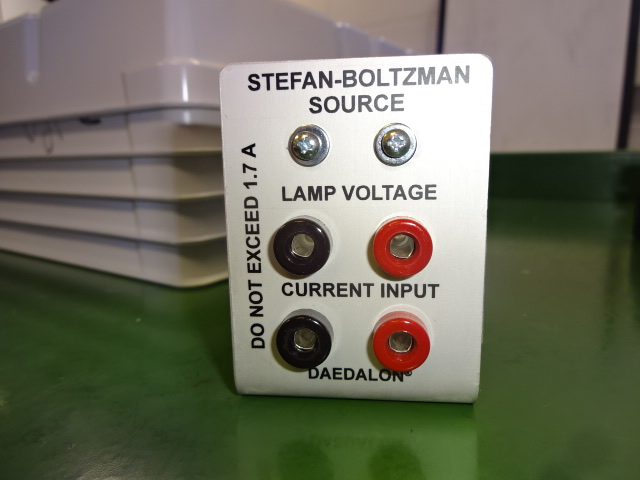
\includegraphics[width=2in]{../images/BulbPanel.jpg}
%}
\caption{The simplified apparatus for the bulb and thermopile, and the bulb's panel.}
\label{fig:apparatus}
\end{centering}
\end{figure}
so that the bulb and thermopile lie on a straight, horizontal line, with a separation of approximately 10 cm.  Connect the bulb's panel to the power supply, and to a voltmeter and ammeter.   

\item Measure the resistance of the filament at a very low current to determine the room temperature resistance.  For a current between 50 and 70 mA, the voltage should be approximately 0.03 V.  

\item \label{sec:PvsT} Investigate the relationship between filament temperature and radiated power. Increase the source voltage in increments of your choice.  {\bf \em Be careful not to exceed 1.7 A through the bulb}.  Record the source voltage and current, and the voltage measured by the thermopile for a variety of data points in this range.  Calculate the filament temperature using Eqn.~\ref{eq-filamenttemp}.   For the thermopile, convert the thermopile output voltage to radiation power (mW) using the conversion factor above. 

\item \label{sec:PvsD}  Investigate the relationship between observed power and distance from the source.   Maintain the filament current at a constant value of your choice  {\bf \em but again not to exceed 1.7 A}.  Vary the distance between the bulb and thermopile in increments of your choice, and record the thermopile output voltage for each distance.   Convert this voltage to radiation power as above. 



%\item Carefully set up apparatus similar to Figure~\ref{fig:apparatus}, 
%\begin{figure}
%\begin{centering}
%\includegraphics[width=5in]{apparatus.jpg}
%\caption{The apparatus.  Note that the specific setup used in the lab does {\em not} have the pivoting arms or the iris diaphram.  Adapt the setup accordingly.}
%\label{fig:apparatus}
%\end{centering}
%\end{figure}
%with the
%but note that our optical bench does not pivot, and we are not using an iris diaphram.  The oven, funnel aperture, and thermopile must all lie on a straight, horizontal line.  The
%oven (on stand) and the funnel aperture are close together. The ceramic
%plug of the power cord is plugged into the oven.  The other end of the
%power cord is plugged into a wall outlet when you are ready to take data.
%The water intake and outflow hoses are attached to the funnel
%aperture as shown.  A slow water flow is maintained throughout the
%experiment.  The digital thermometer probe should be mounted at the
%back of the oven so that as much of the probe's length
%is inside the oven as possible without it touching the oven walls (see
%Figure~\ref{fig:apparatus}).


%The iris, if employed, is 25 cm from the funnel aperture, and the
%thermopile tube is 25 cm from the iris.  However, it may not be
%necessary to include the iris in the setup.)

%\item Set the oven voltage (on the variac) at a constant value ({\em e.g.}\ 110 VAC).  Turn on the variac and measure the oven temperature and

%\item \label{sec:PvsT} Plug the oven in and measure the oven temperature and
%thermopile output voltage at 5 minute intervals for at least 1 hour.  Tabulate
%oven temperature ($T$), time ($t$), thermopile output voltage ($V$) and
%measured radiated power ($P$) in appropriate units. 

%Note:  All the pieces of equipment involved in the above measurements
%must remain motionless during the 60 minutes when the data is recorded.  Continue taking data until the temperature is fairly stable and does not change by more than about a half of a percent over the 5 minutes between readings.

%\item \label{sec:PvsD} With the oven maintained at a constant high temperature, now vary the distance between the funnel aperture and
%the thermopile from 20 cm to 80 cm by steps of 5 cm. 
% (The iris, if employed, should be shifted to mid-positions.)
%Take thermopile output
%voltage readings for each distance. Convert voltage to radiation power
%(mW) using the conversion factor given in the notes on equipment above.
%Tabulate distance $d$ from the funnel aperture source to the thermopile,
%the thermopile output voltage ($V$), and measured radiated power ($P$).
%Also record the oven temperature ($T$).

%\item NOTE: Check with your instructor as to whether Step 4 will be
%carried out or not.
%
%At the same oven voltage and temperature as in Step 2, move the iris and
%thermopile branch of the optical bench through various angles from $\alpha = 0^\circ$ to
%$\alpha = 45^\circ$ in steps of $5^\circ$ each. Measure thermopile
%output voltage for each angular position. Tabulate angle ${\alpha}$,
%thermopile voltage $V$, and measured radiated power $P$. Also record the
%oven temperature $T$.  The distance between the funnel aperture and the
%thermopile must be kept constant for these measurements. 

%Notes:

%\begin{enumerate}
%
%\item Place the thermopile on one of the smaller optical benches for
%this step.  For these measurements, the iris must be used and placed
%midway between the funnel aperture and the thermopile.
%
%
%\item The angle ${\alpha}$ must be carefully determined.  An angular
%scale attached to two rulers is provided and should be placed on the
%table below the optical benches.  The center of the angular scale must
%lie directly below the opening of the funnel aperture.  Each time the
%angle ${\alpha}$ is changed by pivoting the optical bench with the
%thermopile, be sure that the optical benches stay aligned with the
%rulers.  Also, it will be necessary to adjust slightly the position of
%the thermopile; it must be maintained at a constant distance (as read
%on the ruler attached to the angular scale) from the funnel aperture.
%
%\end{enumerate}

\item \label{sec:lesliecube} The intensity of radiation from surfaces with different color and
surface characteristics is studied using Leslie's cube. The instructor will bring a
beaker of water to a boil on a hotplate and (using oven mitts and a
funnel) carefully pour the hot water into Leslie{\textquoteright}s
cube, which is placed on a thermally insulated surface.  Place the
thermopile about 10 cm away from the cube, and measure the radiated
power from each of the 4 vertical surfaces of the cube by measuring the
thermopile output voltage. 

Make sure that the temperature of the cube and the distance (and
relative position) of the thermopile from each cube face are the same
for all of the 4 measurements of the voltage.  The water in the cube
should be stirred with the thermometer or a stirrer to maintain a
uniform temperature at the 4 surfaces. 

Note:  A 6 cm diameter cardboard tube can be used between the cube and
the thermopile to shield the experiment from interference from other
external heat sources, if such interference is present and causes a
problem.

\end{enumerate}

\section{Analysis}

\begin {enumerate}
%\item 
%\begin {enumerate}

%\item For the data of Procedure Step~\ref{sec:PvsT}, plot a graph of temperature
%$T$ (K) as a function of time $t$ (min) using Cartesian axes.  Explain
%qualitatively the shape of this graph.

\item Plot the measured power $P$ (mW) from Step~\ref{sec:PvsT} as a function of
temperature $T$ (K) vs. on Cartesian and on log-log axes. {\em Include error bars on the data points in the graph.} Note that the measured power is proportional to the intensity of the electromagnetic radiation at the position of the thermopile, and thus should also be proportional to $R$, the power/unit area emitted by the oven, treated as a black body. 

What shape should the log-log graph have?  Perform a suitable curve fit
to check the Stefan-Boltzmann law.  Compare your results for the
exponent of $T$ to the mathematical statement of the Stefan-Boltzmann
law.  To what extent have you verified this law?  Discuss, {\em including an estimate of the uncertainty of relevant quantities.}

%\end{enumerate}

\item For the data of Procedure Step~\ref{sec:PvsD}, plot measured power $P$ (in mW) as
a function of distance $d$ (in cm) on Cartesian and log-log axes.  {\em Again, include error bars on the data points in the graph.}  Note
that $P$ is proportional to the intensity of the electromagnetic
radiation at the position of the thermopile.  Perform a suitable curve
fit to check the inverse square law.  Compare the results for the
exponent (of distance $d$) to the mathematical statement of the inverse
square law. To what extent have you verified this law?  Discuss, {\em again including an estimate of the uncertainty of relevant quantities.}


%\item For the data of Procedure Step 4 (if carried out), plot measured
%power $P$ (mW) as a function of cos ${\alpha}$ using Cartesian
%coordinates.  As in step 1b above, $P$ is proportional to $R$, the
%power/unit area emitted by the oven, treated as a black body.  How
%does $R$ vary with the cosine of ${\alpha}$? Discuss.

\item Determine the ratio of the radiated power from each of the four
sides of the Leslie's cube to the radiated power from
the black side of the cube.  Do your results conform to the
predictions of radiation theory?  If there appears to be a discrepancy
between theory and your observations, how might this be explained? 

HINT: For what wavelength range of electromagnetic radiation are your
predictions applicable?  How do those wavelengths compare with the
wavelengths of the radiation emitted by the cube? 

\end{enumerate}

\section{References}
\begin{itemize}
\item Thornton and Rex, Modern Physics $3^{\rm th}$ edition, pp.97-103. 
\item Tipler and Llewellyn, Modern Physics $5^{\rm th}$ edition, pp.119-121. 
\end{itemize}
